\chapter{Segundo prototipo.}
% ----------------------

\label{C:Construcción de modelo final}

\section{Construcción de la fuente definitiva}

A partir de la experiencia obtenida en el desarrollo y las pruebas del primer prototipo de la fuente de tensión, se identificaron varios errores en las huellas y pistas del PCB. Estos problemas fueron corregidos en una nueva versión del diseño, abordando específicamente las fallas detectadas en la etapa inicial. Cada ajuste realizado fue producto de un análisis detallado de las fallas observadas, lo que permitió aprender de los errores y aplicar mejoras sustanciales en esta segunda iteración.\par 
Con esta evolución del diseño, se ha alcanzado el modelo definitivo dentro del marco de este proyecto, logrando cumplir con todos los objetivos planteados desde el inicio. Las funcionalidades establecidas, junto con las mejoras integradas, permiten asegurar que este prototipo final es una solución efectiva y alineada con los parámetros establecidos en la planificación original.\par

\section{Presentación Física.}
Uno de los aspectos distintivos que se abordó en esta versión final de la fuente de alimentación es la optimización de su presentación. El modelo anterior presentado en la figura \ref{F:fuente_anterior} carecía de un diseño compacto y organizado que integrara todos los componentes en un espacio reducido y controlado. Esta carencia no solo dificultaba el traslado del equipo, sino que también exponía sus partes a posibles daños causados por factores ambientales, como humedad, polvo o cambios de temperatura, que podrían afectar negativamente su funcionamiento a largo plazo.\par
Se dio especial atención al desarrollo de un diseño que no solo cumpliera con las especificaciones técnicas y funcionales, sino que también ofreciera una presentación estética y práctica. La disposición interna de los componentes fue planificada para maximizar el uso del espacio disponible, permitiendo una configuración más ordenada y accesible. Además, el gabinete contenedor seleccionado provee una protección robusta contra las condiciones ambientales adversas, asegurando que todos los elementos estén resguardados y puedan operar de manera óptima incluso en entornos desafiantes.\par

\begin{figure}[H]
    \centering
    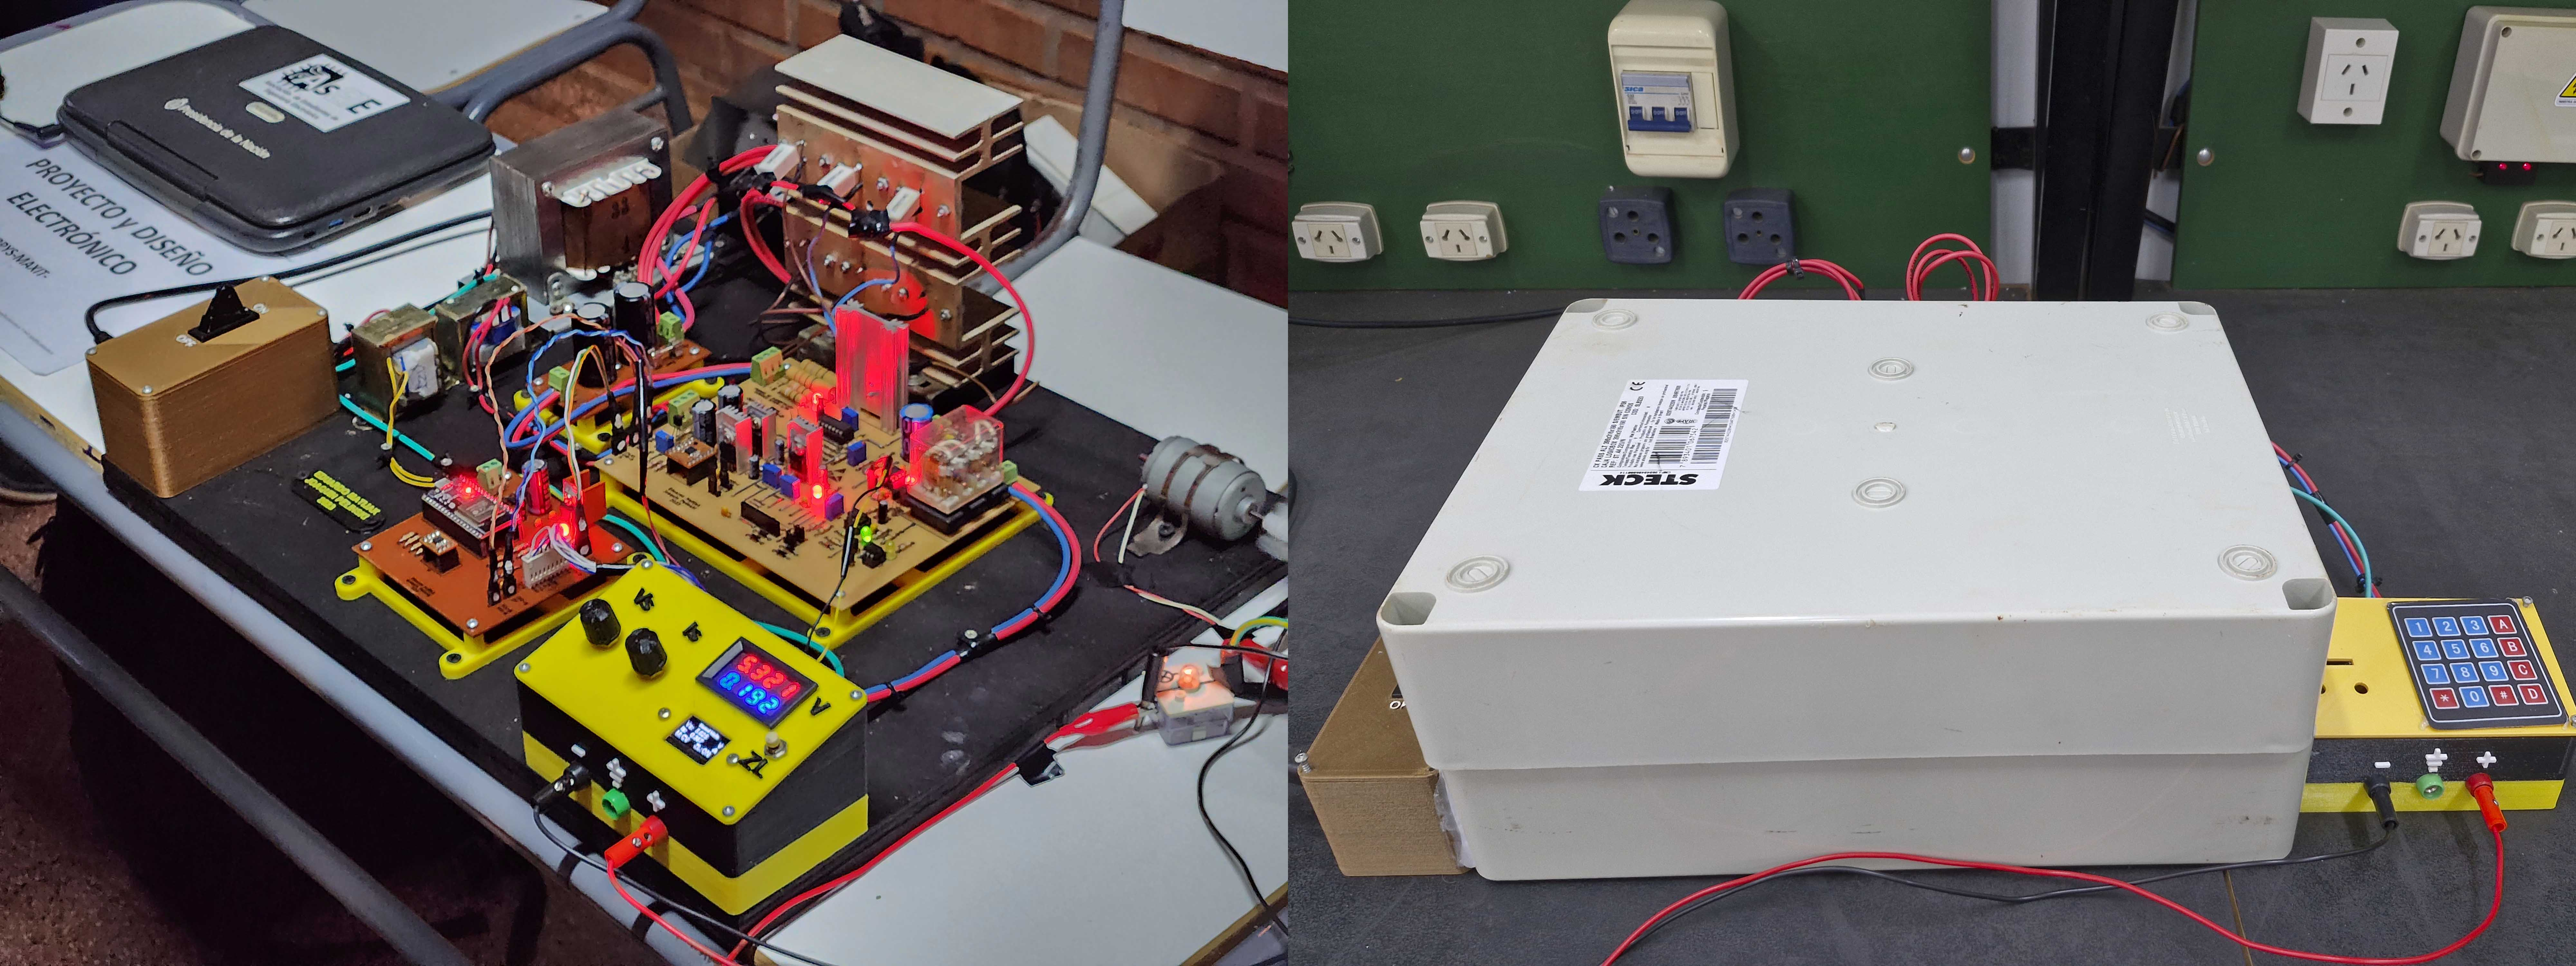
\includegraphics[scale=0.05]{./imagenes/fuente_anterior.jpg}
    \caption{Antes y después de realizada la modernización de la fuente.}
    \label{F:fuente_anterior}
\end{figure}

\subsection{Gabinete contenedor.}
Para la protección y organización de los componentes de la fuente de alimentación, se seleccionó una caja plástica de grandes dimensiones, la cual ofrece tanto espacio adecuado como resistencia estructural. Este gabinete, identificado en la figura \ref{F:gabinete_contenedor}, proporciona una contención segura para la mayoría de los elementos críticos del sistema. En su diseño, se ha dejado espacio en el exterior para el montaje de la pantalla y los controles de configuración, lo que facilita su acceso y manipulación por parte del usuario. Además, el disipador de calor fue montado externamente para optimizar la ventilación y la disipación térmica.\par
Las distintas secciones de la fuente fueron ubicadas estratégicamente, con el objetivo de maximizar el uso eficiente del espacio disponible en el gabinete contenedor, como se muestra en la figura \ref{F:distibucion_gabinete_contenedor}. Se priorizó una disposición organizada y armónica de los componentes y conductores, minimizando el desorden y asegurando una separación adecuada para evitar interferencias o cruces innecesarios entre las conexiones eléctricas.

\begin{figure}[H]
    \centering
    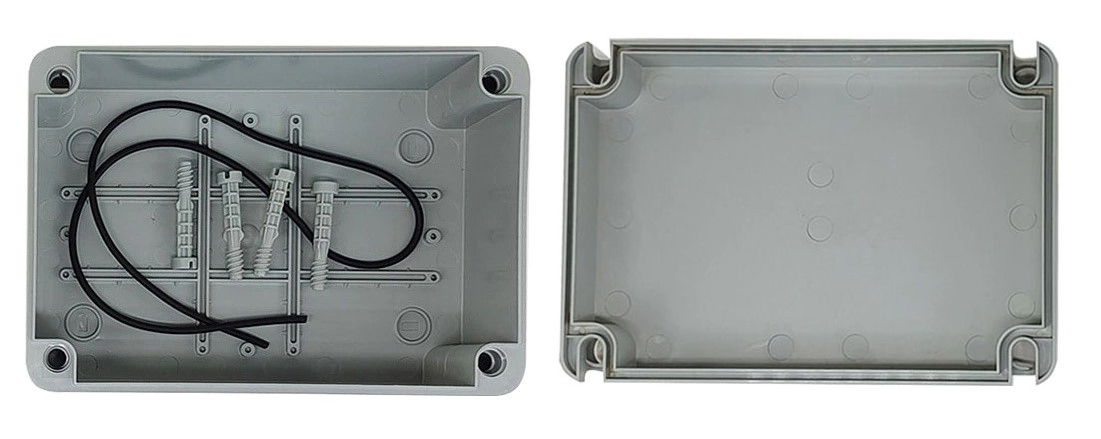
\includegraphics[width=0.8\textwidth]{./imagenes/caja_plastica.jpg}
    \caption{Caja plástica grande - 220×150×90 mm.}
    \label{F:gabinete_contenedor}
\end{figure}

\begin{figure}[H]
    \centering
    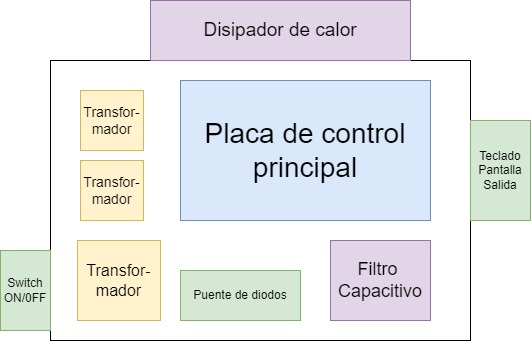
\includegraphics[scale=0.5]{./imagenes/distribucion_secciones.jpg}
    \caption{Distribución de secciones en el gabinete contenedor.}
    \label{F:distibucion_gabinete_contenedor}
\end{figure}

\subsection{Superficie de Montaje Interna}
Para asegurar una base estable y duradera para los componentes electrónicos, se optó por el uso de una superficie de madera forrada, evitando así el montaje directo sobre la caja plástica. Esta solución no solo proporciona una mayor firmeza al atornillar las piezas, sino que también facilita la organización interna y el acceso a los componentes cuando sea necesario realizar ajustes o mantenimientos.\par
La base de madera fue cuidadosamente fijada al fondo del gabinete otorgando bastante estabilidad. Para mejorar aún más la seguridad y la disposición de los circuitos, se diseñaron y fabricaron soportes plásticos mediante impresión 3D como se ve en la figura \ref{F:base3d_fuente}. Estos soportes fueron especialmente diseñados para mantener las placas electrónicas en posición suspendida, evitando el contacto directo con la base y permitiendo que las pistas de cobre y los pines queden al aire, reduciendo el riesgo de cortocircuitos y facilitando el flujo de aire alrededor de los componentes.\par

\begin{figure}[H]
    \centering
    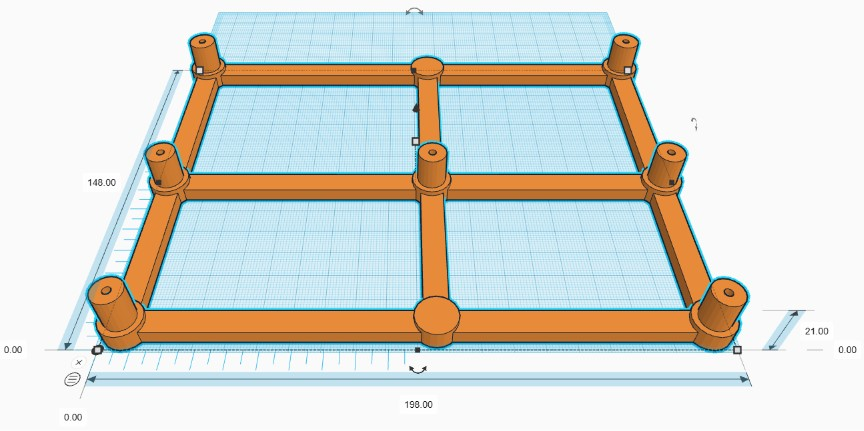
\includegraphics[scale=0.4]{./imagenes/3d_base.jpg}
    \caption{Base plástica 3D para el montaje de la placa de la fuente.}
    \label{F:base3d_fuente}
\end{figure}

\subsection{Sección de interfaz con el usuario}
El componente en cuestión es un pequeño contenedor de color amarillo y negro, ubicado en uno de los laterales del gabinete principal fig \ref{F:caja_usuario}. Este contenedor alberga las bornes de conexión, donde se disponen los terminales que permitirán la vinculación de la carga externa al sistema. \par
Para garantizar una comunicación fluida entre este módulo y el resto de los componentes de la fuente, se ha optado por utilizar un cable de 40 pines. Este tipo de cable, originalmente diseñado para discos duros con interfaz paralela (PATA), resulta ideal para este proyecto debido al elevado número de conexiones necesarias y la robustez que añade a los conductores acoplando todos estos en una sola ficha. En concreto, 16 de estos pines están dedicados a gestionar la comunicación entre el teclado, el encoder y la pantalla, elementos clave en la configuración y monitoreo de la fuente de tensión mientras que el resto de pines no tendrán propósito general y serán asignados a \textit{GND} y a \textit{$V_{CC}$} para fines varios. \par

\begin{figure}[H]
    \centering
    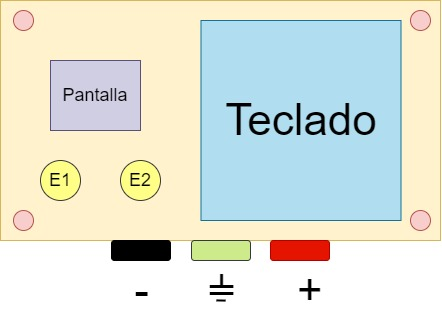
\includegraphics[scale=0.4]{./imagenes/caja_usuario.jpg}
    \caption{Vista superior del panel de control del usuario.}
    \label{F:caja_usuario}
\end{figure}
En base a la necesidad de albergar el teclado, la pantalla y los encoders, se diseñó una tapa en 3D con la disposición indicada en la figura \ref{F:caja_usuario}. \par 
\begin{figure}[H]
    \centering
    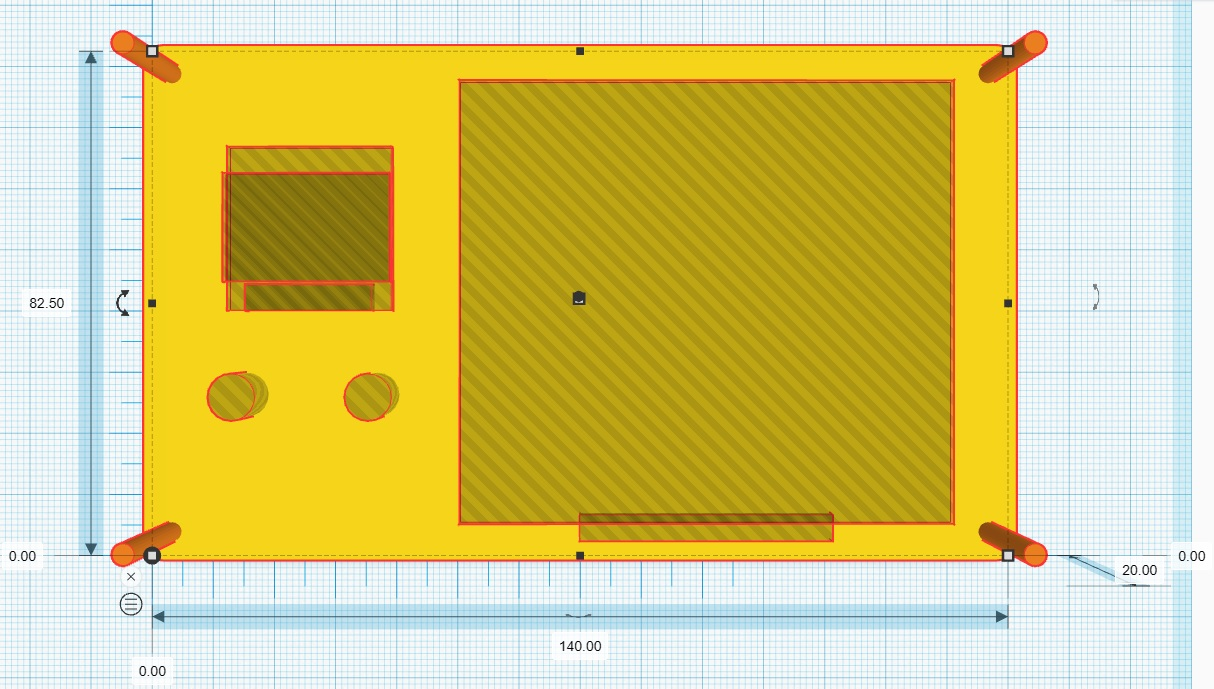
\includegraphics[width=0.6\textwidth]{./imagenes/Tapa_interfaz.jpg}
    \caption{Diseño en 3D de la tapa de la interfaz donde irán montados los módulos.}
    \label{F:Tapa_interfaz}
\end{figure}

\subsection{Correcciones Adicionales}
En esta sección se detallan algunos de los ajustes y correcciones menores que fueron implementados y desarrollados adecuadamente en otras partes del documento. Estos cambios fueron cruciales para optimizar el rendimiento, mejorar la fiabilidad y asegurar la claridad tanto en el diseño físico como en la programación. A continuación, se enumeran los principales aspectos abordados:
\begin{itemize}
    \item \textbf{Ajuste de constantes del controlador:} Se realizaron ajustes finos en las constantes del controlador, lo cual permitió mejorar la precisión y estabilidad del sistema de control. Estos ajustes fueron necesarios para optimizar la respuesta del sistema ante diferentes condiciones de carga y mejorar la robustez del control.
    \item \textbf{Reestructuración del código de programación:} El código de programación del \textit{Arduino Nano} fue reestructurado con el objetivo de optimizar su desempeño, simplificar su lógica y mejorar su comprensión. Esta reestructuración incluyó la eliminación de redundancias, la modularización de funciones clave y la implementación de buenas prácticas de codificación, lo que resultó en un código más eficiente y fácil de mantener.
    \item \textbf{Corrección de huellas PCB de componentes:} Se realizaron correcciones en las huellas PCB de varios componentes para asegurar un ajuste preciso y una correcta conexión en el diseño final. 
    \item \textbf{Redistribución de pistas, pines y componentes:} Se llevó a cabo una redistribución estratégica de las pistas, pines y componentes en el PCB, con el fin de mejorar el flujo de señales, reducir el ruido eléctrico y optimizar el espacio disponible en la placa. Esta redistribución también contribuyó a mejorar la disipación térmica y la accesibilidad para futuras modificaciones o reparaciones.
\end{itemize}

\section{Versión final del PCB}
En base a las correcciones mencionadas en la sección anterior, se presenta en la figura \ref{F:PCB_prototipo2} los PCBs diseñados. En el principal se ha agregado en la parte inferior derecha la sección correspondiente a la conexión con la interfaz de usuario. Fue necesario reubicar el Arduino Nano de forma horizontal para poder enrutar todas las pistas y utilizar la menor cantidad de puentes posibles. \par 
La sección de la derecha corresponde al PCB que se encontrará en la interfaz de usuario. El propósito del mismo será poder distribuir todas las conexiones a los módulos adecuados.
\begin{figure}[H]
    \centering
    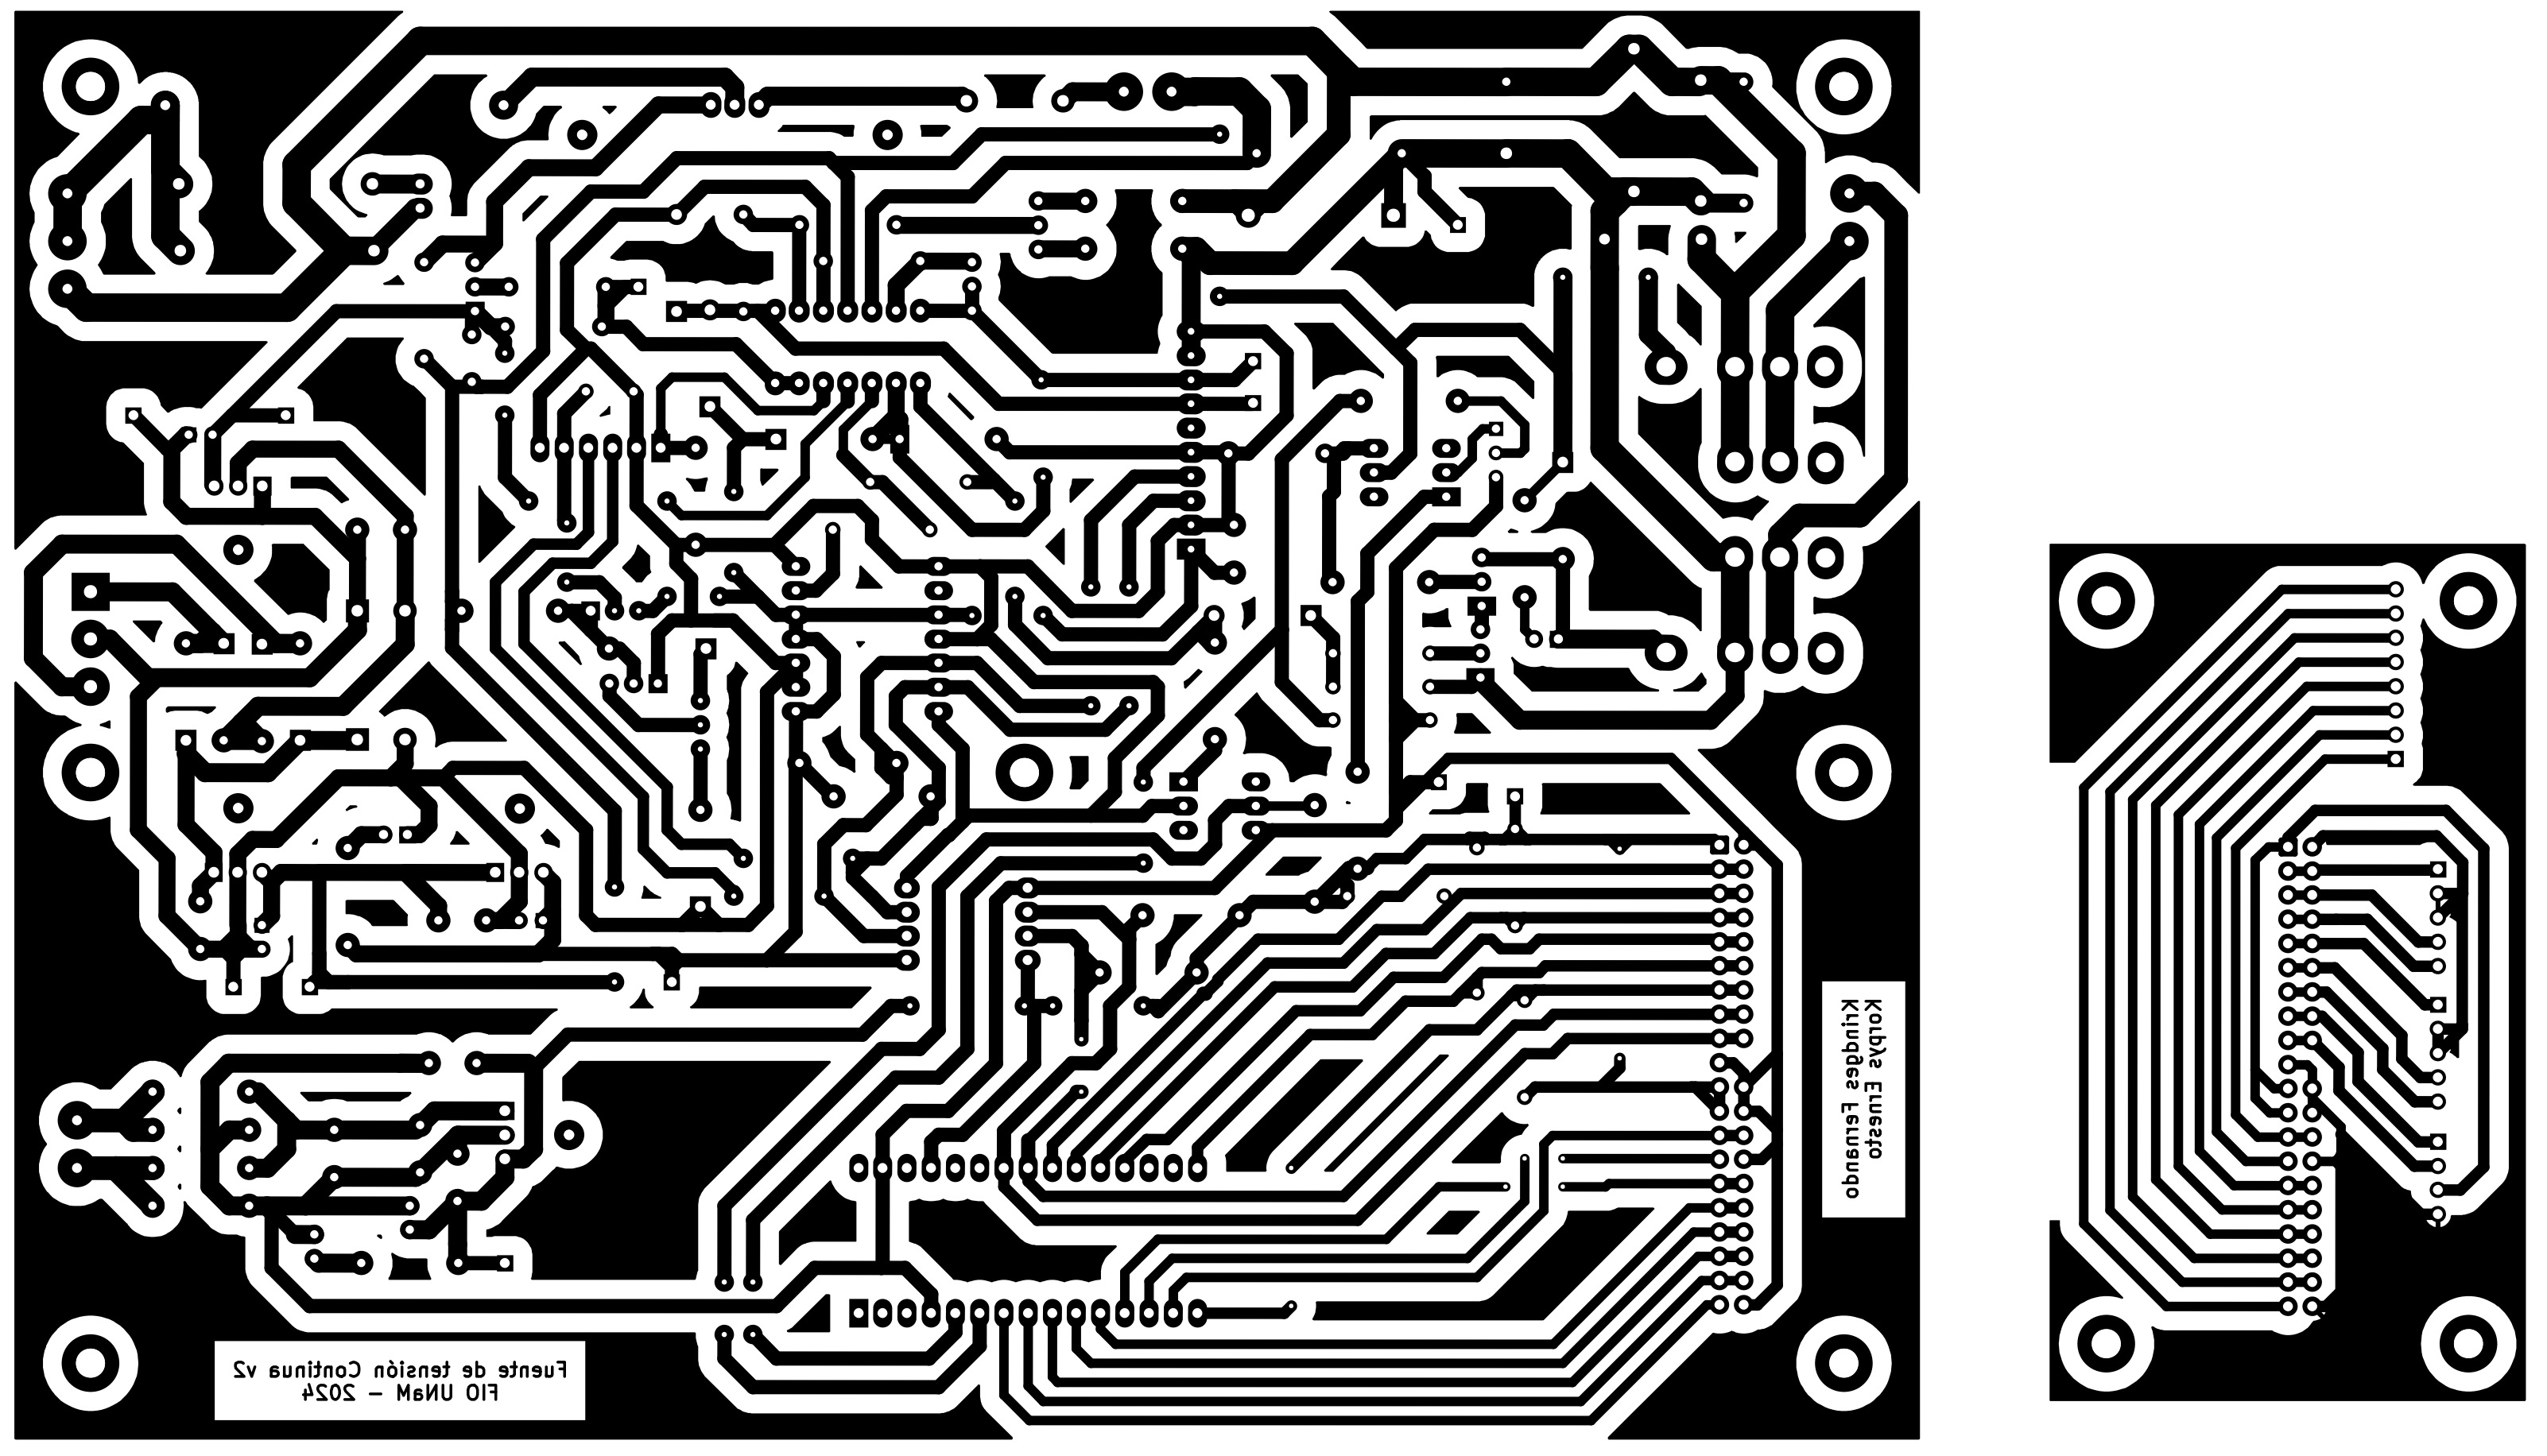
\includegraphics[width=\textwidth]{./imagenes/PCB_prototipo2.jpg}
    \caption{PCB de la fuente de tensión diseñada y de la interfaz de usuario}
    \label{F:PCB_prototipo2}
\end{figure}\par 
Mientras que en la figura \ref{F:3D_v2} se puede observar una vista en 3D de los PCB mencionados.
\begin{figure}[H]
    \centering
    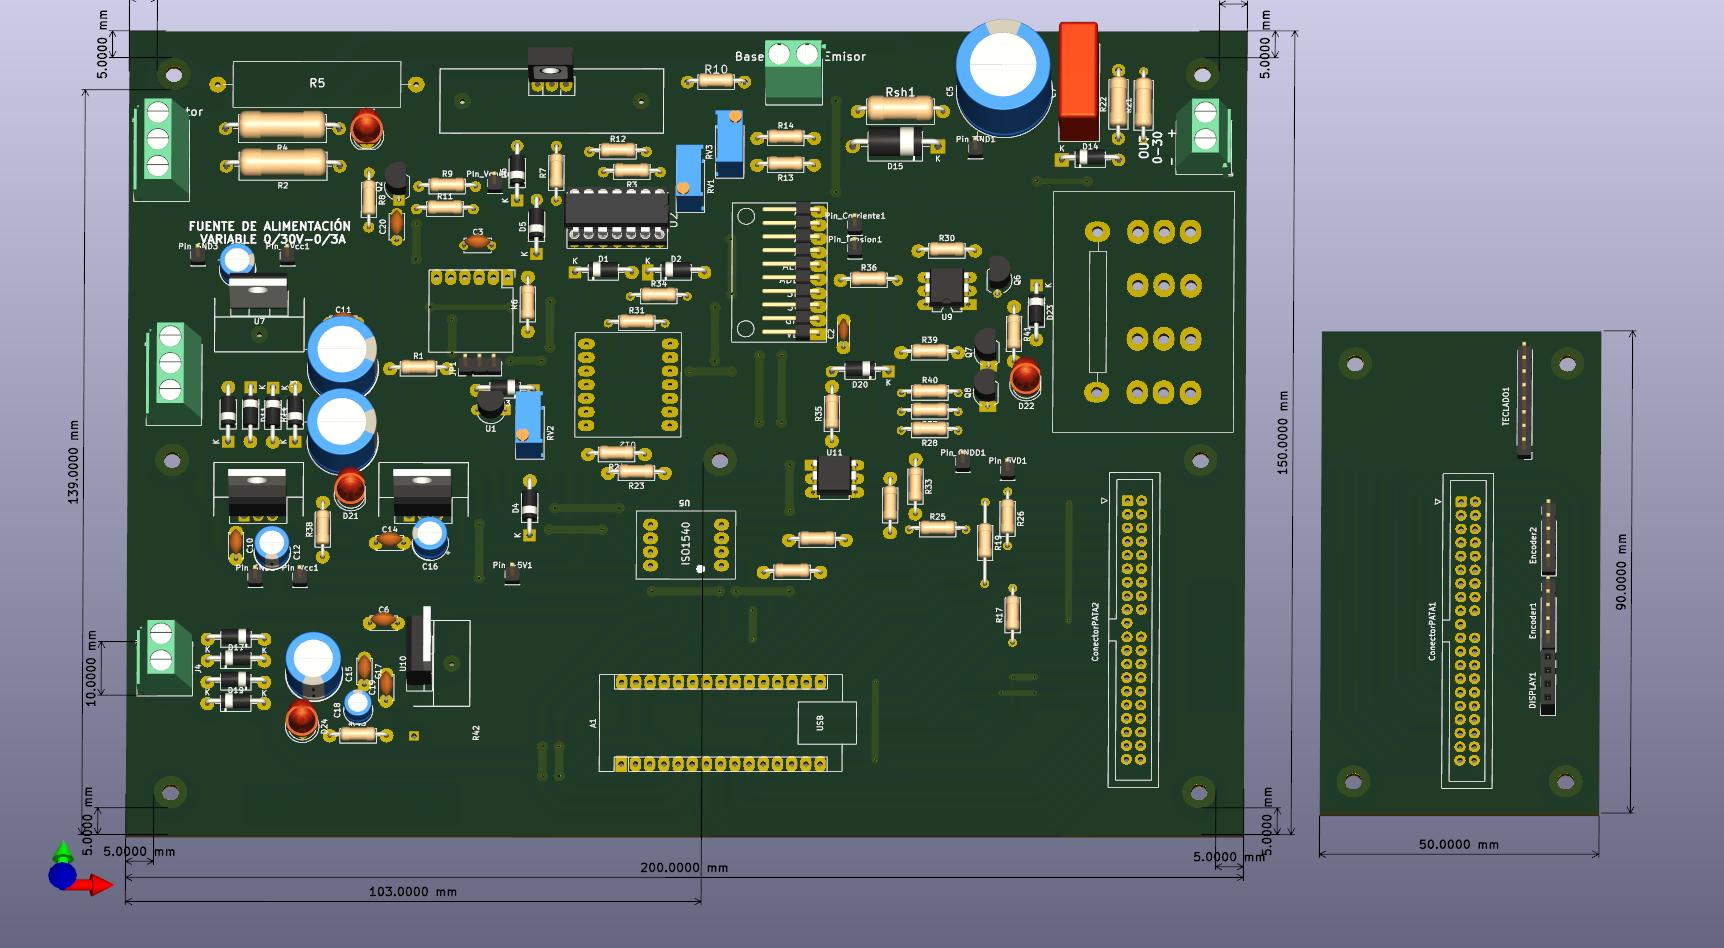
\includegraphics[width=\textwidth]{./imagenes/3D_v2.jpg}
    \caption{Vista en 3D de la versión final del PCB}
    \label{F:3D_v2}
\end{figure}

